\documentclass[12pt]{article}
\usepackage[margin=1in]{geometry}
\usepackage{setspace}
\onehalfspacing

% Start of preamble
%==========================================================================================%

% Required to support mathematical unicode
\usepackage[warnunknown, fasterrors, mathletters]{ucs}
\usepackage[utf8x]{inputenc}

\usepackage[dvipsnames,table,xcdraw]{xcolor}

% Standard mathematical typesetting packages
\usepackage{amsmath,amssymb,amscd,amsthm,amsxtra}
\usepackage{mathtools,mathrsfs,xparse,newtxtext,newtxmath}

% Symbol and utility packages
\usepackage{cancel, textcomp}
\usepackage[mathscr]{euscript}
\usepackage[nointegrals]{wasysym}
\usepackage{apacite}

% Extras
\usepackage{physics}
\usepackage{tikz-cd}
\usepackage{microtype}
\usepackage{enumitem}
\usepackage{titling}
\usepackage{graphicx}

\usepackage{listings}
\usepackage{xcolor}

\lstset{
    basicstyle=\ttfamily\small,
    keywordstyle=\color{blue},
    commentstyle=\color{green},
    stringstyle=\color{red},
    numbers=left,
    numberstyle=\tiny\color{gray},
    breaklines=true,
    frame=single,
    language=Python
}

% Common shortcuts
\def\mbb#1{\mathbb{#1}}
\def\mfk#1{\mathfrak{#1}}

\def\C{\mbb{C}}
\def\R{\mbb{R}}
\def\Z{\mbb{Z}}
\def\cph{\varphi}
\renewcommand{\th}{\theta}
\def\ve{\varepsilon}
\newcommand{\mg}[1]{\| #1 \|}

% Often helpful macros
\newcommand{\floor}[1]{\left\lfloor#1\right\rfloor}
\newcommand{\ceil}[1]{\left\lceil#1\right\rceil}
\renewcommand{\qed}{\hfill\qedsymbol}
\renewcommand{\P}{\mathbb P\qty}
\newcommand{\E}{\mathbb{E}\qty}
\newcommand{\Cov}{\mathrm{Cov}\qty}
\newcommand{\Var}{\mathrm{Var}\qty}

% Sets
\usepackage{braket}

\graphicspath{{/}}
\usepackage{float}

\newcommand{\SET}[1]{\Set{\mskip-\medmuskip #1 \mskip-\medmuskip}}

% End of preamble
%==========================================================================================%

\title{CSE Template}
\date{\today}
\author{Rohan Mukherjee}

\begin{document}
    \maketitle
    \subsection*{Problem 1.}
    \begin{enumerate}[label=(\alph*)]
        \item The best performing stock, which is NVDA, gets a cumulative return of 4.07, while if we were to invest 1/419 in every stock, that would get 0.72. 

        \item For one thing, all our analysis was done assuming that $l_t(i) \in [-1,1]$, so if we work with the unnormalized difference, this wouldn't be satisfied and we couldn't apply the theorem. It also makes more sense to take the relative gain $-(C_{t+1}(i) - C_t(i)) / C_t(i)$ instead of the unnormalized one, because otherwise we do not have a consistent scaling across stocks, meaning that stocks that have huge values (such as Berkshire part A) will dominate the portfolio, and show huge gains even though relatively speaking we haven't made that much money on it. We care about percentage increase, not just absolute increase, because we can only invest \$1 total each day.

        \item From the notes we know that the best $\ve$ is just $\sqrt{\log(n)/T}$. For us, we have $n = 419$ stocks who are the experts, and $T = 1259$ days. So we should pick $\sqrt{\log(419)/1259} = 0.07$. Recall, the multiplicative weights algorithm has gives a regret of $2\sqrt{T \log n}$. For us, is $2\sqrt{1259 \log 419} \approx 174$. Considering how our best performing stock gets a cumulative loss of like 4, this is really bad. We are only required to be within 174 of 4. That's not a very good bound. Presumably our algorithm could give us a return of -170. I don't, however, suspect that we will do this poorly. I would expect that mostly anything that thinks would do better than uniformly sampling each stock, but of course I don't expect it to be anywhere near NVDA. 0.07 means that the weights decay relatively slowly, so it will be fairly close to uniform, so I would suspect it to, although be better, not by very much.

        \item Here is the picture of the cumulative return for multiplicative weights:
        \begin{figure}[H]
            \centering
            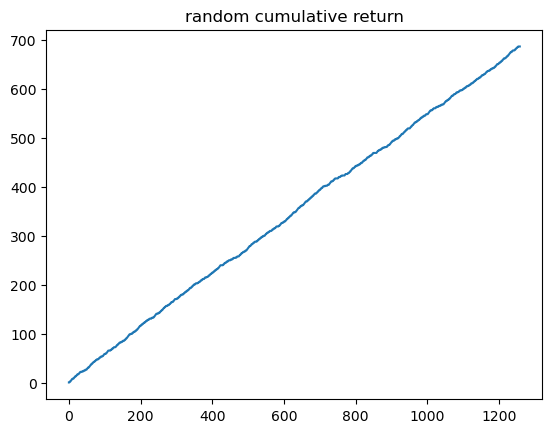
\includegraphics[width=0.8\textwidth]{random_cum_return.png}
        \end{figure}
        In this case, where each price of the stock is independent of all the ones before it, no algorithm will beat purely random in expectation. Let $w_t$ be the weights of the (randomized) algorithm at time $t$. Conditioning on the stock prices beforehand, by independence we have that:
        \begin{align*}
            \E(\sum_{i=1}^n w_t(i) \cdot \frac{C_{t+1}(i) - C_t(i)}{C_t(i)} \bigm| C_1, \ldots, C_t) &= \sum_{i=1}^n w_t(i) \E(\frac{C_{t+1}(i) - C_t(i)}{C_t(i)} \bigm| C_1, \ldots, C_t) 
        \\&= \frac 12 \sum_{i=1}^n w_t(i) = \frac 12.
        \end{align*}
        (Note that we can pull the $w_t(i)$ out of the conditional expectation since it is measurable w.r.t. the $C_1, \ldots, C_t$). Thus given any trading strategy, we are incurring a loss of $-\frac12$ at each time step. So any algorithm does equally well/badly in expectation, so really nothing can be done in this case. Of course even the trivial algorithm does as good as this. Nothing we can do here. Note that we can see above, the best performing stock in hindsight reaches a value of 700 or so, and among 1400 days this is like getting $1/2$ per day, which is what we said would happen in expectation. So there is really no way to beat this, and I think that follows by central limit theorem.

        \item $\ve = 0$ represents when we just don't update the weights at all at each step. We would just take uniform distribution the whole way through. On the other hand, $\varepsilon \to \infty$ would represent just taking the best stock at each time step, and disregarding everything else. Basically it gives the overwhelming majority of the weight to the element that performed best, while completely disregarding everything that performed poorly. This is similar to follow the leader, however follow the leader chooses the best expert based on the expert's total history, while this chooses the best expert based only on the last incremental gain.
    \end{enumerate}
    \subsection*{Problem 2.}
    \begin{enumerate}[label=(\alph*)]
        \item Herre is the graph of the cumulative return with varying $\ve$:
        \begin{figure}[H]
            \centering
            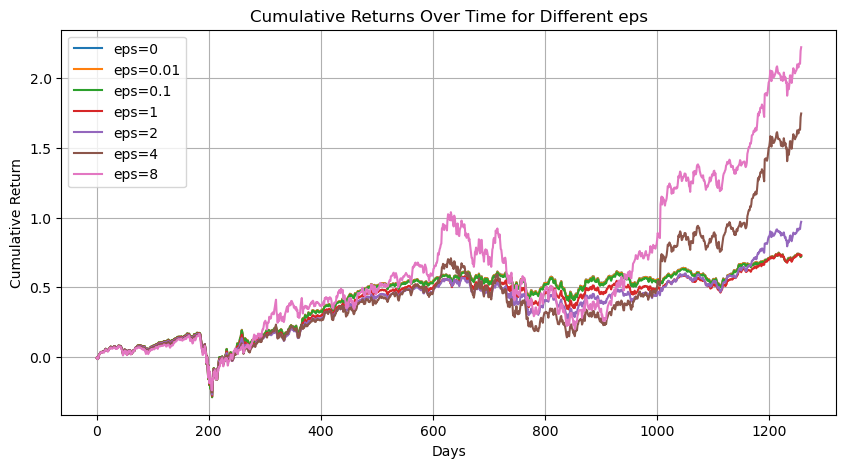
\includegraphics[width=0.8\textwidth]{cum_return_diff_eps.png}
        \end{figure}
        The theoretical best epsilon is $\sqrt{\log(n)/T} = 0.07$. However, you can see  that actually does quite poorly in the above graph. Indeed it even seems like it increases with epsilon. However, the leader among the epsilon changes a lot among the time period. In the real world, NVDA did extremely well in 2024, outperforming every other stock. So following the leader in that case would give us a great final return. For us, this is most simulated by $\ve = 8$, and by the theoretical discussion before will be more and more like this with $\ve \to \infty$. Because of this we see the final value increasing with $\ve$. However, throughout the middle, whichever stock was the leader caused gigantic losses for the $\ve = 8$ curve, highlighting the risky strategy. We can also see that the $\ve = 0.1$ curve, representative of the right $\ve$ (0.07 is closer to 0.1 than to 0.01) is the most stable. This is likely correlated with the theoretical guarantees. I would not have suspected 0.07 to be the best $\ve$, because while that gives the best theoretical bound, it is not necessarily the best trading strategy for multiplicative weights. That's not a well-posed question and can be answered in a number of different ways. 

        \item Here is the graph of the multiplicative weights diversity versus epsilon:
        \begin{figure}[H]
            \centering
            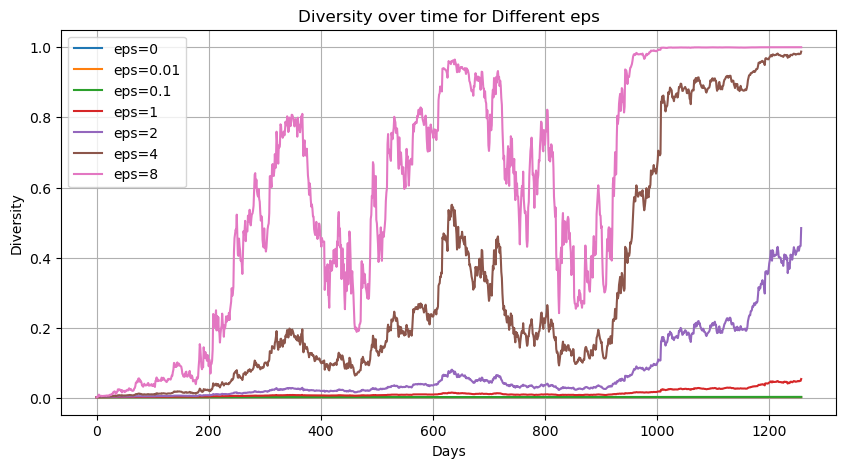
\includegraphics[width=0.8\textwidth]{diversity_graph.png}
        \end{figure}
        As you can clearly see, at the end and throughout the middle, $\ve = 4,8$ seem to be putting a huge amount of weight on one particular stock. Especially 8, near the end it is just putting almost everything on NVDA. The same happens near the end for $ve = 4$ as well. You can also see this behavior to a much smaller extent with $\ve = 2$, which seems to have good diversity throughout until around day 1000, where it starts to invest more and more into one stock. What is curious, is that the other $\ve = 0, 0.01, 0.1$ and 1 to an extent, except near thet end, all have very good diversity. There are no huge spikes, whatsoever. This is again related to our discussion above, about how $\ve \to \infty$ will just pick the best performing stock from the last day. 

        \item Here is the graph without NVDA:
        \begin{figure}[H]
            \centering
            \includegraphics[width=0.8\textwidth]{cum_return_diff_eps_no_NVDA.png}
        \end{figure}
        Here is the graph of the diversity without NVDA:
        \begin{figure}[H]
            \centering
            \includegraphics[width=0.8\textwidth]{diversity_graph_no_NVDA.png}
        \end{figure}

        Wow, absolutely remarkable. Just by removing one stock the end cumulative return vs epsilon totally flips behavior. Now the smaller $\ve$ are doing the best. Since the cash cow NVDA is gone, the risky strategies $\ve \geq 4$ are now doing noticably worse than all the low-risk ones $\ve \leq 2$. The final value goes from increasing in $\ve$ to decreasing in $\ve$. From a philisophical standpoint, I find this very amusing. You can do all this complicated math and yet just investing equally into all 419 stocks does the best. Now, the best $\ve$ becomes $0.1$ which is closest to our $0.07$, which is what we were expecting. This is remarkable. Also, for the diversities, the $\ve = 8$ curve still seems to really prioritize one stock, with probablities very frequently above 0.6. However unlike lsat time, it never goes all the way to 100\%, and doesn't stay constantly 100\% at the end. On the the other hand, very high max probabilities effect on $\ve = 2$ is greatly reduced. In this case, $\ve = 1$ is much more stable, and once again $\ve = 0.1, 0.01, 0$ they are basically fully diverse. No huge spikes or investment in any of them. NVDA was really fueling big gains for the risky strategy!

        \item As stated above, I don't think that multiplicative weights is a particularly good strategy for investing. $\ve = 0.07$, is so small, that it gets like the same performance as just investing $1/419$ in every stock. That second strategy would let me sleep much more peacefully at night. On the other hand, if I had a huge expectation that the market would turn bullish, and that some stocks would start flying, I would certainly use the multiplicative weights strategy. As we saw, when one stock vastly out performs the rest it actually works really well. And this algorithm could find it without me even having to look into any stocks. Yet this strategy is extremely risky, hugely validated by how bad $\ve = 8$ does without its cash cow NVDA. Another issue is that the current market price is not simply a function of the past. Recently, the administration put huge tariffs on canada and mexico, which sent stocks plummetting. This algorithm would say that GM, Stellantis, and the other car companies are very bad, and we should divest from them. But what it couldn't tell from the price is that the President would lift tariffs on specifically automobiles, sending their stocks flying upwards. Since there are just so many outside variables, this method is not robust enough. It doesn't use anywhere near enough information. 

        \item The model in theory treats all losses equally over time. Indeed, at time step $s$, the total loss incurred by our algorithm is
        $$\sum_{t \leq s} E_{i \sim p_t}(l_t(i)).$$ In particular, independent of $t$ the coefficient of $E_{i \sim p_t}(l_t(i))$ is the same. However, it does make sense to treat recent losses more heavily. The performance of the stock is much more relevant to the recent past than the distant past. For example, if a penny stock got a giant government contract, and exploded 100x in value, it's changes when it was still a penny stock aren't symbolic of how its going to do anymore. So we really shouldn't be worried about that loss as much, we should be caring more about the recent losses. I propose the following fix to this. Instead of incurring the loss $E_{i \sim p_t}(l_t(i))$, at time step $t$, I say we should incur $E_{i \sim p_t}(tl_t(i))$, so the loss gets bigger with time. This way we are more sensitive to recent losses.

        \item I acknowledge that this is not real investment advice and I won't try it with my own money.

        \item So I tried the above, and it didn't work that well. Instead, if $l_t$ is the loss vector at time step $t$, and $\ell = \min |l_t|$, the update rule I used was $w_{t+1}(i) = w_t(i)^{1-\ve \ell} e^{-\ve l_t(i)}$. Since $1-\ve \ell < 1$, it basically takes a very small root, hence giving exponential decay to the older losses. I tried what I did above and it just wasn't very good. This had more promising results though! Here is the graph of cumulative return for this time sensitive scheme vs $\ve$:
        \begin{figure}[H]
            \centering
            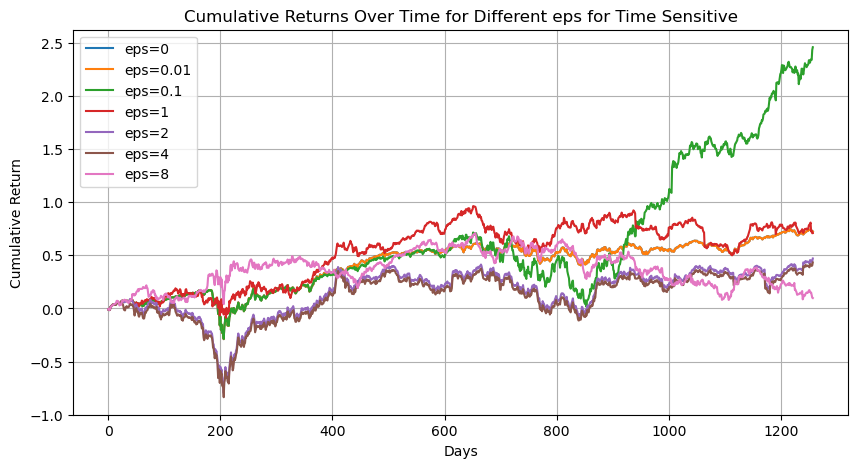
\includegraphics[width=0.8\textwidth]{cum_returns_diff_eps_time_sensitive.png}
        \end{figure}
        As you can see, our optimal $\ve = 0.1$ now does as good as 2.5, even better than $\ve = 8$ from way before! I find this remarkable. It also does noticably better than literally everything else. This method is surely super sensitive to the $\ve$ value. You will also notice that $\ve = 2,8,0.1$ avoided the covid crash, while $\ve = 2,4$ totally got crushed. I am not sure why this happens and why it doesn't happen with increasing $\ve$. This strategy isn't super stable in that sense. Here is the diversity graph:
        \begin{figure}[H]
            \centering
            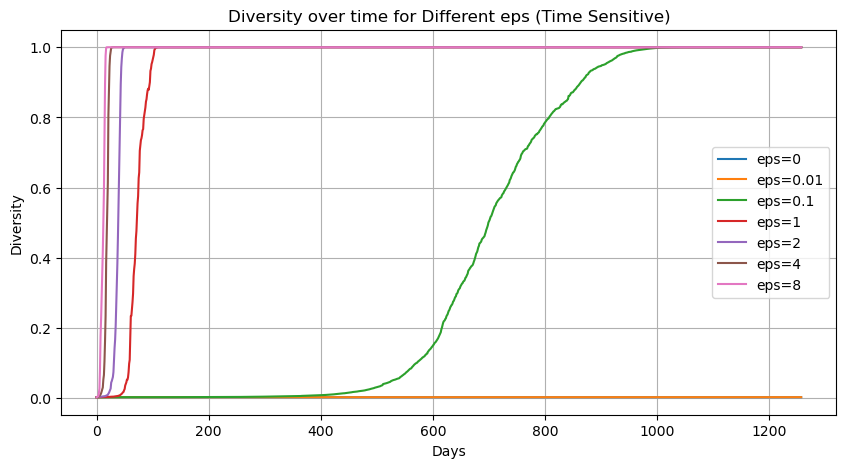
\includegraphics[width=0.8\textwidth]{diversity_graph_time_sensitive.png}
        \end{figure}
        It seems like $\ve = 0.1$ only commits to a strong stock once it has seen it do well for a long time. This is exactly the behavior I would want from an investment strategy. However it is unfortunate that it invests all 100\% into one stock at the end. But the other cases, $\ve = 0.01,0$ do not fuel gains basicaly at all. They are way too safe. 
        On the other hand, without NVDA, we get:
        \begin{figure}[H]
            \centering
            \includegraphics[width=0.8\textwidth]{cum_returns_diff_eps_time_sensitive_no_NVDA.png}
        \end{figure}
        Whose diversity graph looks like this:
        \begin{figure}[H]
            \centering
            \includegraphics[width=0.8\textwidth]{diversity_graph_time_sensitive_no_NVDA.png}
        \end{figure}
        Remarkably, this is the same graph as before. The green found a stock that constantly performs strongly, decided it had seen it long enough, and fully comitted to it, fueling HUGE gains. The stock it found was KLAC, and with a look at its actual performance, I can see why it fueled so many gains. I think it is hard for the other more sensitive $\ve$ to escape 100\%, since they are have basically no weight at all on anything else. That is why this fully commit strategy is good for $\ve = 0.01$. Throughout both graphs, $\ve = 0.1$ is able to mostly avoid the covid recession. That's quite interesting, but at the end, I'm not sure how well it would do. It is again a really risky strategy since it is pouring all its money onto just one stock, but at the same time it is fueling huge gains. It is extremely interesting to me that it was able to find a second well performing stock like NVDA to fuel huge gains, albeit definitely smaller. 
    \end{enumerate}
\end{document}